\documentclass{ctexart}
\title{黑盒优化与概率推断}
\author{姚兴虎}
\date{\today}

\usepackage{geometry}
\geometry{a4paper,scale=0.8}
\usepackage{amsfonts}
\usepackage{amsmath}
\usepackage{amssymb}
\usepackage{graphicx}
\usepackage{subfig}
\usepackage{dsfont}
\newtheorem{Def}{\hspace{2em}定义}
\newtheorem{Theo}{\hspace{2em}定理}
\usepackage{cite}
\begin{document}
	
\maketitle
\section{黑盒优化}
\subsection{几种优化问题的例子}
\subsubsection{线性回归的最小二乘解}
给定数据集$D={(\mathbf{x}_1,y_1),(\mathbf{x}_2,y_2),\cdots,(\mathbf{x}_m,y_m)}$,其中$\mathbf{x}_i =(x_{i1};x_{i2};,\cdots,x_{id}),y_i \in \mathbb{R}.$ “线性回归”试图学得一个线性模型以尽可能准确地预测实值输出标记,即线性回归试图学的如下的线性函数
\begin{equation*}
f(\mathbf{x}_i=\boldsymbol{\omega}^T\mathbf{x}_i + b),
\end{equation*}
使得$f(\mathbf{x}_i)\simeq y_i$.我们记$\hat{\boldsymbol{\omega}}=(\boldsymbol{\omega};b)$,相应的,把数据集$D$表示为一个$m\times(d+1)$大小的矩阵$\mathbf{X}$,其中每行对应于一个样本,该行的前$d$个元素对应于样本的$d$个属性值,每个样本的最后一个属性横置为1,然后把标记也写为向量形式$\mathbf{y}=(y_1;y_2;\cdots;y_m)$.若矩阵$\mathbf{X}^T\mathbf{X}$为满秩矩阵或正定矩阵,令$\hat{\mathbf{x}}_i=(\mathbf{x}_i,1)$则我们可以求出线性回归问题的解析表达式如下所示:
\begin{equation*}
f(\hat{\mathbf{x}}_i) = \hat{\mathbf{x}}(\mathbf{X}^T\mathbf{X})^{-1}\mathbf{X}^T\mathbf{y}.
\end{equation*}


可以看出对于简单的线性回归问题,我们可以求出其最优解的解析表达式.能求出一个优化问题最优解的解析表达式意味着一方面我们在全局范围内找到了这一优化问题的全局最优解,另一方面我们可以避开迭代算法等计算代价相对庞大的近似求解算法(在这里只考虑最简单的线性回归问题,不考虑矩阵不可逆的情形,也不考虑矩阵求逆的计算量).\cite{周志华2016机器学习}
\subsubsection{反向传播与梯度算法}
线性模型,例如线性回归和逻辑回归,由于其能够求出其解析解或者使用凸优化算法进行迭代找到最优解,因此在很多问题上得到了广泛的应用.然而,线性模型也有很致命的缺陷,那就是模型的表达能力被限制的线性函数里,所以其无法拟合输入和输出之间的非线性映射关系.可以通过将线性模型作用在输入属性的一个非线性变换后的结果$\phi(\mathbf{x})$上或者通过核方法、手工构造的方法以及深度神经网络的方法来构造隐含的非线性映射.


神经网络函数与线性模型的一个重要区别在于其非线性结构使得多数我们感兴趣的代价函数变得非凸。这意味着我们对这类问题的优化求解通常采用迭代的基于梯度的优化,仅仅使得代价函数达到一个非常小的值;而不是像线性模型那样求解其最优解的解析表达式或像逻辑回归和支持向量机那样设计一个全局收敛的迭代算法。深度网络中的反向传播算法没有全局收敛性保证并且往往对迭代初始点的选择敏感。优化深度网络模型的方法大多是对最简单的梯度下降算法的改进。各种算法都利用了代价函数梯度的一步步反向传播从而迭代地优化神经网络的权重值.\cite{goodfellow2016deep}

\subsubsection{神经网络中的超参数调整}
神经网络中除了需要优化网络的权重值,其他比如网络的类型(如全连接网络、卷积神经网络、循环神经网络),损失函数中的超参数设置(如正则化系数的设置),网络的初始化策略,优化迭代方法的选择都对最后的性能有着非常大的影响。这些参数不能通过反向传播算法进行优化,我们常常将其称为超参数。模型的性能关于超参数的不可微性使得梯度算法难以用来对超参数进行优化,简单的对超参数进行的网格搜索算法和随机搜索算法需要耗费大量的代价(大量的计算资源消耗和大量的金钱成本)。我们从以下三点阐述寻找一个自动化对神经网络中超参数进行优化的方法具有很大的研究价值:(1)减少在应用机器学习算法中人的参与.这样可以将人类从繁琐的调参过程中解放出来,大大降低优化一个深度网络的工作量.(2)提升机器学习算法的性能.通过参数优化技术有望找到更优的超参数配置从而提高机器学习算法的性能。(3)提高机器学习算法的可复现性以及不同算法之前比较的公平性。大量的机器学习算法通过在特定任务上的精心调参使得其在当前任务获得极好的性能,这一方面使得复现这一实验结果比较困难,另一方面不同的算法性能的比较似乎受限于不同研究人员的调参水平。因此通过统一的参数调试方法的构建可以提高机器学习算法的可复现性以及算法之间比较的公平性。


超参数的自动选择具有很大的吸引力然而其作为优化问题的高度复杂性使得设计一个有效的优化方法十分困难.(1)评估函数的计算代价十分昂贵.在深度学习中的训练过程需要一个庞大的数据集并且网络往往拥有庞大的参数规模,这使得对超参数的单独一组值的性能评价就非常昂贵.(2)不同超参数的取值情况十分复杂.可以是正则化参数这种连续值,网络的深度以及每层的单元数这种整数值,也可以是是否采用dropout这种二值数据,也可以是采用何种优化方法这种集合数据.(3)我们通常不能求得性能函数关于超参数的梯度信息.这也就是说,我们通过在传统优化问题中用到的性质比如凸性和光滑性无法在这一类问题中使用.(4)当训练数据集规模较小时,我们无法对算法的泛化误差进行优化.\cite{automl}\cite{feurer_hyperparameter_2018}
\subsection{何为黑盒优化}
非形式化的来说,一个黑盒函数$f$可以理解为从$\mathbb{R}^n$到$\mathbb{R}$的一个映射.但是映射关系$f$的解析表达式及工作方式未知,我们只能通过不断地将数据输入到黑盒函数中然后通过得到的输出值来猜测黑盒函数的结构信息.下图表示一个黑盒问题的映射关系.
\begin{figure*}[htb!]
	\centering
	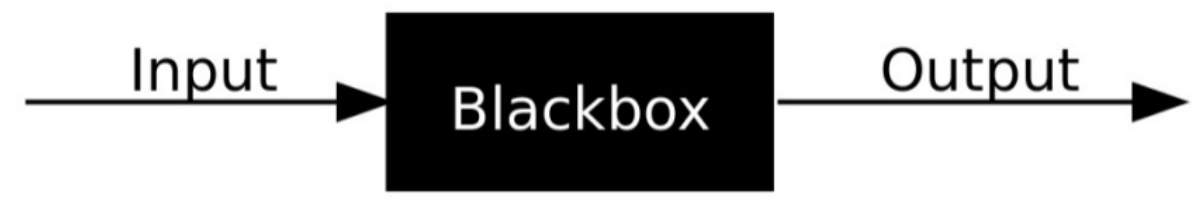
\includegraphics[scale=0.5]{blackbox.png}
	\caption{黑盒函数示意图}
\end{figure*}


与黑盒优化问题相对应的优化问题便是白盒优化问题。白盒问题要么优化问题的具体形式已知(如线性回归和SVM),要么虽然表达式的形式未知,但是我们可以利用目标对优化参数的梯度进行迭代(如深度网络,尽管深度网络也常被看做一个黑盒).这里的黑盒优化指的是优化目标的具体表达式及其梯度信息均未知的优化问题,因此我们无法利用优化目标的本身特性求得其全局最优解,也无法直接利用参数的梯度信息.


除了深度网络的超参数优化问题之外,深度强化学习中智能体与环境的交互问题也可以看做一个黑盒优化问题.在model-free强化学习问题中,我们不对智能体所处的环境进行建模.在这种情形下,我们将环境当做一个黑盒,智能体通过不断尝试动作来从这个黑盒中获得奖励值,最后的优化目标是使累计获得的奖励值最大.下图展示了强化学习问题的一般步骤.\cite{sutton2018reinforcement}
\begin{figure*}[htb!]
	\centering
	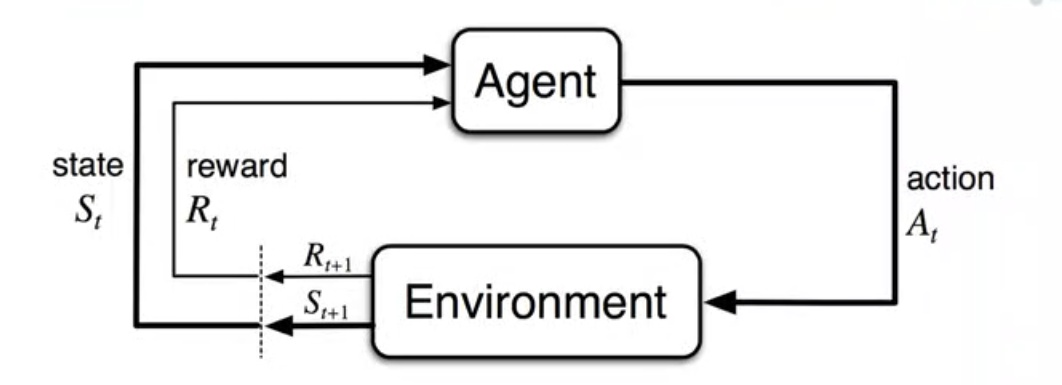
\includegraphics[scale=0.45]{reinforcement.jpg}
	\caption{强化学习示意图(无模型强化学习问题中的环境是一个黑盒).}
\end{figure*}
\subsection{黑盒优化的简单方法}
\subsubsection{网格搜索法与随机搜索法}
网格搜索(grid search)是最基本的黑盒优化方法,其也被称为全因子设计(full factorial design).用户为每一个要优化的参数执行一个有限的值集,然后在这些参数的笛卡尔积所构成的网格上进行性能评估.因为需要评估的次数随参数数量的增加呈现指数增长,因此这种方法很难被用到参数数量多的高维黑盒优化场合.此外我们若对网格取得非常密集(每个参数对应的取值集合的基数过大),则在参数数量不多的情形下也需要庞大的计算代价.\cite{automl}

\begin{figure*}[htb!]
	\centering
	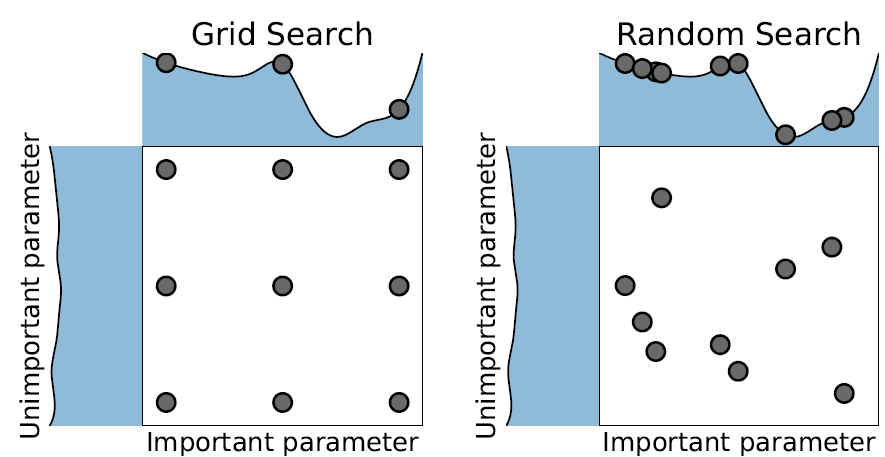
\includegraphics[scale=0.55]{search.png}
	\caption{当模型中有一个重要参数和一个不重要参数时网格搜索和随机搜索的比较(可以看出同样是进行9次性能评估,随机搜索能够搜索更多的重要参数上所对应的值).}
\end{figure*}
一个简单的可以替代网格搜索的方法是随机搜索(random search)法.顾名思义,随机搜索在参数的可能取值中随机抽出来进行性能评估,知道我们给定的计算资源耗尽为止.当其中一些参数比另一些参数重要得多时,随机搜索算法往往比网格搜索方法更有效.只管上来说,当我们对$N$个参数总共进行$B$次性能评价时,网格搜索只能对每个参数只能评价其在$B^{1/N}$个位置上的性能,而随机搜索则能对每个点都评估其取$B$个不同值的性能.这一示意图如下所示.


由于随机搜索算法没有对机器学习算法进行任何假设并且在给定足够的计算资源的情况下其能够逼近模型的最优解,因此其是评价一个黑盒优化算法的一个有用的基准线.随机搜索算法常常与更复杂的优化算法相结合来提升算法的收敛速率以及增加模型的探索性.由于随机优化算法能够对整个参数空间进行搜索,因此其常被用来初始化一些更为复杂的算法.

其他黑盒优化的方法有遗传算法,进化算法等基于种群的算法.


\subsection{机器学习中的不确定性}
\subsubsection{何为不确定性}
我们标准的回归和分类模型不能够捕捉到不确定性来介绍机器学习问题中面临的不确定性.在分类任务中,模型输出的高概率值(如softmax输出的高概率值)往往被错误的解释为模型对当前分类结果的置信度.事实上,一个具有极大概率输出值的模型依然可能具有很高的不确定性.如下图所示的一个理想化的二分类任务,训练数据全部处于图中的两条竖着的灰色虚线之间,那么在阴影区域由于并没有训练样本所以在这一区域我们无法对估计的函数值进行调整.尽管分类器在点$x^*$处以概率1判断其属于类别1,但是由于其处于模型的不确定区域中,因而其输出具有很高的不确定性.\cite{gal2016dropout}
\begin{figure*}[htb!]
	\centering
	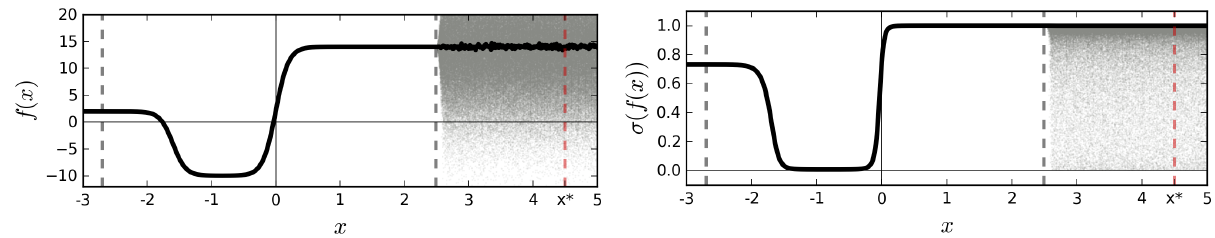
\includegraphics[scale=0.5]{uncertainty.png}
	\caption{一个理想二分类问题的softmax的输入函数$f(x)$和输出函数$\sigma(f(x))$(训练样本集中在两条竖虚线之间,灰色区域代表由于没有训练样本所以无法对曲线$f(x)$进行调整的不确定性区域. $x^*$表示不确定区域中的一个点,在这一点,分类器以概率1输出其属于类别1).}
\end{figure*}


在这个例子中,对模型的测试中出现了与训练数据偏差较大的数据,由于并没有与在这些未见过的数据的范围内对模型进行训练,从而不能够保证模型能够给我们一个值得信赖的分类结果.总的来说,主要有以下几个方面会使得模型预测的结果呈现不确定性:(1)噪声数据.我们的观测数据是带有噪声的,这可能是由于测量误差或者其他可能影响观测的因素导致的.在噪声数据上对模型进行拟合会给模型的预测带来不确定性.(2)模型参数的不确定性.众多机器学习算法尤其是深度学习算法,其模型会有大量的参数,并且不同的参数组合都能够很好的拟合训练数据.我们去选择那种参数的组合去实际应用其实面临模型参数的不确定性问题.(3)模型结构的不确定性.我们无法判断我们应该使用何种网络结构来使得模型更能适应当前的问题.


在模型给出分类结构的同时给出其对当前结果的不确定性置信度是十分重要的.这是因为在一些诸如疾病检测和自动驾驶等领域,当机器学习算法做出决策时还应给出当前决策可能所面临的风险,因此从这种观点来看,对机器学习模型不确定性的研究属于人工智能安全性的研究范围.
\subsubsection{黑盒优化问题中的不确定性}
黑盒优化问题其巨大的计算代价限制了其训练数据的规模,因此如何根据模型的不确定程度来指导我们对模型性能进行更为有效的评估至关重要.贝叶斯优化理论是对黑盒问题进行全局优化并且给出模型不确定性的一种前沿方法,其有两个关键的组成部分:一个概率代理模型(probabilistic surrogate model)和一个确定下一步评估哪个点的获取函数(acquisition function).在每次迭代中,通过目前位置所有的观测值对代理函数进行拟合.然后根据概率模型的预测分布来确定不同候选点对减少模型不确定性所起到的作用来权衡对当前模型的探索与利用(是通过采样新的数据来进一步降低模型的不确定性还是利用当前的模型进行预测).与需要昂贵评估代价的黑盒函数相比,这里的获取函数的计算成本较低,从而可以对该获取函数进行优化.
下图是通过高斯过程代理函数来对一个一维问题进行贝叶斯优化的例子.我们的目标是使得阴影范围(模型的不确定性)尽量小.途中显示我们通过优化获取函数找到其一个最优值来影响后续的数据点的采样情况.(关于该例子的更详细介绍参见参考文献\cite{gal2016uncertainty})
\begin{figure*}[htb!]
	\centering
	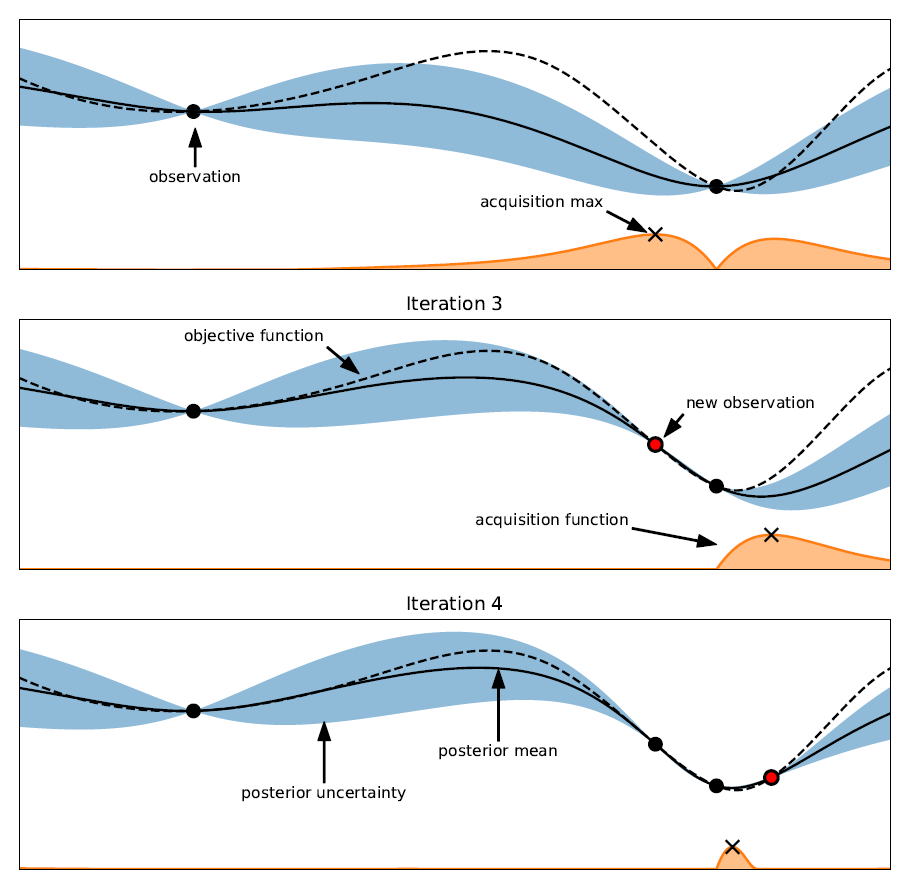
\includegraphics[scale=0.6]{bayesin.png}
	\caption{一维函数上的贝叶斯优化过程示例.}
\end{figure*}


\subsection{高斯过程与不确定性}

\subsubsection{随机过程}
\begin{Def}
随机过程:设$(\Omega,\mathcal{F,P})$为一概率空间,另设集合$T$为一指标集合.如果对于所有$t\in T$,均有一随机变量$\xi_t(\omega)$定义于概率空间$(\Omega,\mathcal{F,P})$,则集合$\{\xi_t(\omega)|t\in T\}$为一随机过程.
\end{Def}

在随机过程中的指标集合$T$常常是时间的集合.因此随机过程常常被用来描述随时间变化的随机现象比方说:人一生中身高的变化,股票在一天中的价格变化,某路段一天的车流量变化等.如果指标集合$T$至多可列,那么称为离散时间;如果$T$是一个实数区间,则称为连续时间.随机过程可分为:离散时间离散状态,离散时间连续状态,连续时间离散状态,连续时间连续状态.


\subsubsection{高斯过程}
高斯过程的相关定义如下.
\begin{Def}
若随机过程$\xi_t(\omega)$的任意$n$维$(n=1,2,\cdots)$分布都是正太分布,则称该随机过程为高斯随机过程或正态过程.
\end{Def}
\begin{Theo}
	$\{\xi_t(\omega)|t\in T\}$是高斯过程的充要条件是其任意有限多个元素的线性组合是正态随机变量.
\end{Theo}
\begin{Theo}
设已给指标集合$T=[0,+\infty)$,实值函数$m(t)$及对称非负定的二元实值函数$K(s,t),s,t\in T$,则存在概率空间$(\Omega,\mathcal{F,P})$及定义在其上的实正态过程$\{\xi_t(\omega)|t\in T\}$,其均值为$m(t)$,协方差矩阵为$K(s,t)$.
\end{Theo}
\begin{Def}
	称随机过程$\{\xi_t(\omega)|t\in T\}$为独立过程,如对任意$n$及$t_1,t_2,\cdots,t_n\ge 0,$随机变量$\xi_{t_1}(\omega),\xi_{t_2}$\\$(\omega),\cdots,\xi_{t_n}(\omega)$相互独立.
\end{Def}
并且我们有,
\begin{Theo}
	正态过程$\{\xi_t(\omega)|t\in T\}$独立的充要条件是$K(s,t)=0,s\ne t.$
\end{Theo}


高斯过程是一个用来度量模型不确定性的很好的工具,其在贝叶斯优化理论中起着至关重要的作用,前文提到的利用高斯过程进行一维函数上的贝叶斯优化就是一个很好的度量模型不确定性的一个例子.
%\subsection{基于高斯过程的贝叶斯黑盒优化方法}
%\subsubsection{贝叶斯优化方法}

%\subsubsection{贝叶斯黑盒优化}
\section{黑盒变分推断}
%\subsection{变分推断}
\subsection{从EM算法讲起}
设计概率模型的一个中心任务是如何通过给定的观测数据来计算潜在变量(隐变量)的后验概率分布$p(\mathbf{Z|X})$,以及计算这一概率分布的期望.这里的模型中可能由一些固定的参数,我们可以不对这些参数进行考虑;模型也可能是一个纯粹的贝叶斯模型,其中所有的未知参数都有一个先验概率分布并且被整合到了隐变量的集合中,记为$\mathbf{Z}$.


期望最大化算法(Expectation Maximization Algorithm,EM),是一种迭代算法,可用于求解含有隐变量的概率参数模型的最大似然估计或最大后验估计。对观测变量为$\mathbf{X}$,隐变量为$\mathbf{Z}$,模型参数为$\boldsymbol{\Theta}$的隐变量模型中的参数$boldsymbol{\Theta}$进行最大似然估计应该最大化如下的对数似然
\begin{equation*}
LL(\boldsymbol{\Theta}|\mathbf{X,Z}) = \text{ln}p(\mathbf{X,Z}|\boldsymbol{\Theta}).
\end{equation*}
然而由于$\mathbf{Z}$是隐变量,上式无法直接求解.此时我们可以通过对$\mathbf{Z}$计算期望,来最大化一观测数据的对数"边际似然"
\begin{equation*}
LL(\boldsymbol{\Theta}|\mathbf{X}) = \text{ln}p(\mathbf{X}|\boldsymbol{\Theta}) = \text{ln}\sum_{\mathbf{Z}}p(\mathbf{X,Z}|\boldsymbol{\Theta})
\end{equation*}
EM算法是一种通过迭代来估计参数隐变量的方法,其基本思想是:若参数$\boldsymbol{\Theta}$已知,则可根据训练数据推断出最优隐变量$\mathbf{Z}$的值(E步);反之,若$\mathbf{Z}$的值未知,则可方便地对参数$\Theta$做极大似然估计(M)步.于是,以初始值$\boldsymbol{\Theta}^0$为起点,对上式可迭代执行以下步骤直至收敛\\
1) 基于$\boldsymbol{\Theta}^t$推断隐变量$\mathbf{Z}$的期望,记为$\mathbf{Z}^t$;\\
2) 基于已观测变量$\mathbf{X}$和$\mathbf{Z}^t$对参数$\Theta$做极大似然估计,记为$\Theta^{t+1}$;\\
这就是EM算法的原型.简要来说,EM算法使用两个步骤交替计算:第一步是期望E步,利用当前估计的参数值来计算对数似然的期望值;第二步是最大化M步,寻找能使E步产生的似然期望最大化的参数值.然后,新得到的参数值被重新用于E步,直至收敛到局部最优解.EM算法在无监督聚类和概率PCA等问题的求解上有着十分重要的应用.
\subsection{变分推断}
一些较为简单的问题我们可以通过EM算法进行解决,但是实际应用中的许多问题我们无法计算后验概率的分布或者计算该后验分布的期望.并且在连续变量的情形下,需要求解的积分往往没有解析解,并且空间维度和被积函数的复杂程度使得整个数值积分的数值解也变得不可行.在这里我们需要借助近似方法.根据近似方法依赖于随机近似和确定性近似,我们可以将近似方法分为两大类:以马尔科夫链蒙特卡洛(MCMC)为代表的随机近似方法和以变分推断(variational inference)为代表的确定性近似方法.


变分的方法起源于18世纪的欧拉,拉格朗日.假设我们由一个纯粹的贝叶斯模型,其中每个参数都有一个先验概率分布.我们把所有潜在变量和参数组成的集合记做$\mathbf{Z}$,将所有观测变量的集合记为$\mathbf{X}$.例如,我们可能有$N$个独立同分布的数据,其中$\mathbf{X}=\{x_1,x_2,\cdots,x_N\}$且$\mathbf{Z}=\{z_1,z_2,\cdots,z_N\}$.我们的概率模型确定了联合概率分布$p(\mathbf{X,Z})$,我们的目标是找到对后验概率分布$p(\mathbf{X,Z})$以及模型证据$p(\mathbf{X})$的近似.由于$p(\mathbf{X}) = \frac{p(\mathbf{Z})p(\mathbf{X|Z})}{p(\mathbf{Z|X})}$我们可以将对数边缘概率进行分解,得到
\begin{align*}
lnp(\mathbf{X}) &=\mathcal{L}(q)+KL(q\|p)
\end{align*}
其中,
\begin{align*}
\mathcal{L}(q) &= \int q(\mathbf{Z})ln\left\{\frac{p(\mathbf{X,Z})}{q(\mathbf{Z})}\right\}d\mathbf{Z}\\
KL(q\|p) &= -\int q(\mathbf{Z})ln\left\{\frac{p(\mathbf{Z|X})}{q(\mathbf{Z})}\right\}d\mathbf{Z}
\end{align*}
我们可以通过关于概率分布$q(\mathbf{Z})$的最优化来使变分下界(evidence lower bound,ELBO)$\mathcal{L}(q)$达到最小值,这等价于最小化KL散度.如果我们允许任意选择$q(\mathbf{Z})$,那么下界的最大值出现在KL散度等于0的时刻,此时$q(\mathbf{Z})$等于后验概率分布$p(\mathbf{Z|X})$.然而当需要处理的模型对真实概率分布的操作不可行时,我们便要考虑$q(\mathbf{Z})$的一个受限制的类别.限制近似概率分布的一种方法是使用参数概率分布$q(\mathbf{Z}|\omega)$,它由参数集合$\omega$控制.这样变分下界变成了$\omega$的函数,我们可以利用标准的非线性最优化方法确定参数的最优值.假设变分分布是一个分量独立的高斯分布往往能够对我们的问题带来简化.\cite{bishop2006pattern}
\subsection{简单变分推断的缺陷}
对一些特定的模型,其条件分布具有计算方便的形式并且其存在方便的变分族函数(如变分线性回归和变分逻辑斯蒂回归中的共轭函数),这种情况下我们可以采用变分推断的一般方法进行优化求解.然而对于更一般的模型和任意的变分分布,普通的变分推断方法就无法进行有效求解了.针对不同的模型我们可以设计模型特异性的求解方法,但是针对具体的问题设计特定的求解策略是一个费事费力的工作,下面将要介绍的黑盒变分推断则能够对复杂多样的模型与概率分布进行近似.
%\subsubsection{贝叶斯神经网络}

\subsection{黑盒变分推断}
\subsubsection{黑盒变分推断的基本原理}
在概率模型中,们把所有潜在变量和参数组成的集合记做$\mathbf{Z}$,将所有观测变量的集合记为$\mathbf{X}$.我们用由参数$\lambda$控制的变分分布$q(\mathbf{Z}|\lambda)$来近似后验概率$p(\mathbf{Z|X})$.变分推断中我们优化如下的ELBO
\begin{equation*}
\mathcal{L}(\lambda) = \mathbb{E}_{q_{\lambda}(\mathbf{Z})}\left[lnp(\mathbf{X,Z})-lnq(\mathbf{Z})\right]
\end{equation*}
最大化ELBO等价于最小化变分分布与后验分布的KL散度,为了通过随机优化方法来优化ELBO,我们需要一个ELBO梯度的无偏估计这样我们便可以通过对样本的采样来进行优化.我们对ELBO关于参数$\lambda$求导可得
\begin{align*}
\nabla_{\lambda}\mathcal{L} &=
\nabla_{\lambda}\int (lnp(\mathbf{X,Z})-lnq(\mathbf{Z}|\lambda))q(\mathbf{Z}|\lambda)d\mathbf{Z}\\&=
\int \nabla_{\lambda}[(lnp(\mathbf{X,Z})-lnq(\mathbf{Z}|\lambda))q(\mathbf{Z}|\lambda)]d\mathbf{Z}\\&=
\int\nabla_{\lambda}[lnp(\mathbf{X,Z})-lnq(\mathbf{Z}|\lambda)]q(\mathbf{Z}|\lambda)d\mathbf{Z}+\int\nabla_{\lambda}q(\mathbf{Z}|\lambda)(lnp(\mathbf{X,Z})-lnq(\mathbf{Z}|\lambda))d\mathbf{Z}\\&=
-\mathbb{E}_{q}[lnq(\mathbf{Z}|\lambda)]+\int\nabla_{\lambda}q(\mathbf{Z}|\lambda)(lnp(\mathbf{X,Z})-lnq(\mathbf{Z}|\lambda))d\mathbf{Z}\\&=
0+\int\nabla_{\lambda}q(\mathbf{Z}|\lambda)(lnp(\mathbf{X,Z})-lnq(\mathbf{Z}|\lambda))d\mathbf{Z}\\&=
 \mathbb{E}_{q}\left[\nabla_{\lambda}lnq(\mathbf{Z}|\lambda)(lnp(\mathbf{X,Z})-lnq(\mathbf{Z}|\lambda))\right]
\end{align*}
然后我们便可以在变分分布中进行蒙特卡洛采样来对上述梯度进行估计,估计方法如下
\begin{equation*}
\nabla_{\lambda}\mathcal{L} \simeq \frac{1}{S}\sum_{s=1}^{S}\nabla_{\lambda}\text{ln}q(\mathbf{Z}_s|\lambda)(\text{ln}p(\mathbf{X,Z}_s)-\text{ln}q(\mathbf{Z}_s|\lambda)),\quad \mathbf{Z}_s\sim q(\mathbf{Z}|\lambda).
\end{equation*}
于是,我们可以利用随机优化方法得到如下的迭代更新公式
\begin{equation*}
\lambda = \lambda + \rho \frac{1}{S}\sum_{s=1}^{S}\nabla_{\lambda}\text{ln}q(\mathbf{Z}_s|\lambda)(\text{ln}p(\mathbf{X,Z}_s)-\text{ln}q(\mathbf{Z}_s|\lambda))
\end{equation*}
值得注意的是,这里的采样仅仅依赖于变分分布而不依赖模型的隐藏结构.因此我们可以构建多种变分分布然后打包起来用在多种模型的优化中.\cite{ranganath2014black}
\subsubsection{黑盒变分推断中的方差控制}
我们可以直接用上面的方法来最大化ELBO,但是上面算法通过蒙特卡洛采样对梯度进行估计可能会产生较高的方差从而使得算法不稳定.解决这一问题的最简单的方法就是调小学习速率,但是这又会导致算法的收敛过慢的问题.我们在这里介绍一种通过Rao-Blackwellization来进行方差削减的方法.


Rao-Blackwellization方法通过将随机变量的期望变为关于随机变量子集的条件期望来进行方差消减.这常常需要真毒不同的问题对这一条件随机变量的积分表达式进行解析求解.在这里我们可以通过采样的方法绕过这一解析求解的过程.在最简单的情形中,Rao-Blackwellization方法通过将一个二元随机变量概率密度函数替换为一个变量对另一个变量的条件分布来进行期望的求解.考虑随机变量$X$和$Y$,和一个概率分布函数$F(X,Y)$.我们的目的是求解$X$和$Y$所构成的联合概率分布的期望$E(J(X,Y))$.


定义$\hat{J}(X) = E(J(X,Y)|X)$,从而有$E[\hat{J}(X)] = E[J(X,Y)]$.这意味在蒙特卡洛近似中,$\hat{J}(X)$可以替代$J(X,Y)$来近似$E(J(X,Y))$.这一近似的方差为
\begin{equation*}
	\text{Var}(\hat{J}(X)) = \text{Var}(J(X,Y)) - E[(J(X,Y)-\hat{J}(X))^2]
\end{equation*}
这意味着$\hat{J}(X)$比原始的估计$J(X,Y)$具有更小的方差.从而我们可以将这一方法利用到黑盒优化过程中去进行方差控制.文献\cite{ranganath2014black}中还介绍了一种易于实现的控制变量方法用来降低算法的方差.


在这里我们介绍一种在变分自编码器中用到的重参数化(Reparameterization trick)方法来优化黑盒变分推断的ELBO
\begin{equation*}
\mathcal{L}(\lambda) = \mathbb{E}_{q_{\lambda}(\mathbf{Z})}\left[lnp(\mathbf{X,Z})-lnq(\mathbf{Z})\right]
\end{equation*}
重参数技巧将一个随机变量$\mathbf{Z}\sim q_\phi(\mathbf{Z|X})$表示为给定$X$后由另一个随机变量$\boldsymbol{\epsilon}$经过一个确定函数$g_\phi$映射得到的,从而有
\begin{equation*}
\mathbf{Z} = g_\phi(\mathbf{X},\epsilon),\quad \epsilon\sim p(\boldsymbol{\epsilon})
\end{equation*}
其中分布$p(\boldsymbol{\epsilon})$独立于$\mathbf{X}$和$\phi$并常常选取为对角高斯分布.在这一情况下,我们可以将对分布$q_\phi(\mathbf{Z|X})$求期望转换为对分布$p(\epsilon)$求期望,即可以推导出如下的公式
\begin{align*}
	\nabla\mathbb{E}_{q_\phi(\mathbf{Z|X})}[f(X,Z)] &= \nabla\mathbb{E}_{p(\epsilon)}[f(X,g_\phi(X,\epsilon))]\\
	&=\mathbb{E}_{p(\epsilon)}[\nabla f(X,g_\phi(X,\epsilon))]
\end{align*}
将上述公式应用到变分推断的ELBO中,黑盒变分法的ELBO的梯度可以写为如下形式
\begin{align*}
\nabla_{\lambda}\mathcal{L}(\lambda) &= \nabla_\lambda\mathbb{E}_{q_{\lambda}(\mathbf{Z})}\left[lnp(\mathbf{X,Z})-lnq(\mathbf{Z})\right]\\
&= \nabla\mathbb{E}_{p(\epsilon)}[lnp(\mathbf{X,Z})-lnq(\mathbf{Z})]\\
&= \mathbb{E}_{p(\epsilon)}[\nabla_\phi g_\phi(\mathbf{X},\epsilon)\nabla_\mathbf{Z}(lnp(\mathbf{X,Z})-lnq(\mathbf{Z}))]
\end{align*}
这一简单的重参数化技巧可以使得我们从一个噪声分布中进行采样从而获得对梯度的无偏随机估计.更重要的是,在连续隐变量模型中,这一简单的方法比其他估计方法具有更小的方差.\cite{louis2017areview}
\subsubsection{黑盒变分推断的缺陷}
变分推断问题需要推断出后验分布$q(Z|X)$,由于每个数据都要被模型所利用,因此这一方法的模型参数会随着样本数量的增加线性增长,在大样本问题上往往需要较高的计算代价;其次便是对于未见过的样本,该模型无法直接进行推断,该模型无法伴随着新样本的出现动态调整,而只能够将新的样本加入到旧样本中重新计算后验分布.
\subsection{利用隐式模型来近似推断}
\subsubsection{隐式模型}
随着变分推断的发展,隐式概率模型也引起了人们的兴趣.这可以归功于生成对抗网络(GAN)的引入及其在生成清晰图像,合成真实的自然语言文本以及解决其他类似问题方面取得的空前成功.


隐式模型仅根据模拟器或生成过程中的某种形式来指定,生成过程可以产生对某种现象的观测值.与机器学习中普遍存在并且长期建立的显式概率模型相比,隐式模型没有指定对模型中的潜在变量进行概率密度的显式建模.


虽然隐式模型可能更笨拙和难以训练,但是其在处理具有更高密度和更高保真度的物理现象时更有潜力.实际上,隐式模型在物理,工程和自然科学领域中无处不在.他们被广泛的应用到生态学,高能物理学,气候科学,地质学等领域.在这些领域中,我们用一个模拟器来模拟真实世界的观测值,从而预测结果.在这里,我们介绍一种利用生成对抗网络来对概率推断问题进行建模的方法.
\subsubsection{隐式模型用于变分推断}
一个对ELBO进行优化的方法是直接对概率比的对数进行优化,这一方法的最直接方法就是利用一个生成对抗网络进行优化,我们用一个概率分类的例子来解释这一方法.我们构建一个概率分类器$t(\mathbf{x})$来区分当前的样本$\mathbf{x}$是来自与分布p还是来自于分布q(在这里我们可以任务分布q是真实的后验分布,分布p是我们的估计值).我们记$t(\mathbf{x}) = \sigma(r(\mathbf{x})$是一个函数$r(\mathbf{x})$后面输出接到一个sigmoid函数上用作对当前样本是来源于真实分布还是近似分布的一个判别器.我们可以利用下面的损失函数来训练这一分类器
\begin{equation*}
	\mathcal{F}_{\text{GAN}}(r,q) = \mathbb{E}_{p(\mathbf{x})}[\text{log}\sigma(r(\mathbf{x}))]+\mathbb{E}_{q(\mathbf{x})}[\text{log}(1-\sigma(r(\mathbf{x})))]
\end{equation*}


GAN的目标是通过求解下面优化问题的一个鞍点来学得一个隐式分布q的估计$r(\mathbf{x})$
\begin{equation*}
	\min_{q\in \mathcal{Q}}\max_{r_\in\mathcal{R}}\mathcal{F}_{\text{GAN}}(r,q)
\end{equation*}
我们可以看出当$r(\mathbf{x})$取真实的对数概率比$r*(\mathbf{x}) = \text{log}p(\mathbf{x})-\text{log}q(\mathbf{x})$时,$\mathcal{F}_{\text{GAN}}(r,q)$可以达到最大值.因而我们可以利用$r(\mathbf{x})$来作为媒介去求解真实的对数密度比.\cite{mohamed2016learning}
\bibliographystyle{plain}
\bibliography{ref}
\end{document}